\section{پروژه دوم (بخش اول): پیاده‌سازی و آموزش شبکه‌ی عصبی (CNN) پایه}

در این بخش از پروژه، هدف ما طراحی، آموزش و ارزیابی یک شبکه‌ی عصبی پیچشی اختصاصی از پایه (\lr{Training from Scratch}) برای دسته‌بندی ۱۷ کلاس مختلف از گل‌ها است. این کار به ما کمک می‌کند تا یک خط پایه (\lr{Baseline}) برای مقایسه با روش‌های پیشرفته‌تر مانند یادگیری انتقالی (\lr{Transfer Learning}) به دست آوریم.

\vspace{0.4cm}
\subsection{آماده‌سازی مجموعه داده و پیش‌پردازش}

مجموعه داده‌ی \lr{17-Flower} شامل تصاویر متنوعی از گل‌هاست. برای جلوگیری از بیرون‌زدگی متن و مدیریت بهتر حافظه، از ابزار بارگذاری مستقیم کراس یعنی
\lr{image\_dataset\_from\_directory}
استفاده کردیم. تصاویر با ابعاد استاندارد $224 \times 224$ پیکسل به سه بخش مجزا تقسیم شدند:

\begin{stepbox}
\field{توزیع داده‌ها و مدیریت حافظه}{
\begin{itemize}
    \item \textbf{داده‌های آموزش (\lr{Train}):} $952$ تصویر
    \item \textbf{داده‌های اعتبارسنجی (\lr{Validation}):} $238$ تصویر
    \item \textbf{داده‌های آزمون (\lr{Test}):} $170$ تصویر
\end{itemize}
\vspace{0.2cm}
برای افزایش سرعت آموزش، از تکنیک‌های \lr{Cache} و \lr{Prefetch} در خط لوله‌ی داده (\lr{Data Pipeline}) استفاده شد تا پردازشگر گرافیکی (\lr{GPU}) در انتظار بارگذاری داده‌ها از دیسک نماند.
}
\end{stepbox}

\vspace{0.4cm}
\subsection{تحلیل عمیق معماری مدل پیشنهادی}

قلب تپنده‌ی این بخش، معماری شبکه‌ی پیچشی است که برای استخراج ویژگی‌های بصری گل‌ها طراحی شده است. به دلیل حجم محدود داده‌های آموزشی، از همان ابتدا لایه‌ی \lr{Sequential} برای \lr{Data Augmentation} در ورودی شبکه تعبیه شد تا با چرخش، زوم و انتقال تصادفی، مدل را در برابر تغییرات محیطی مقاوم کند.

در شکل \ref{fig:model_summary}، خلاصه‌ی لایه‌ها و پارامترهای این شبکه را مشاهده می‌کنید. 

\begin{figure}[h!]
    \centering
    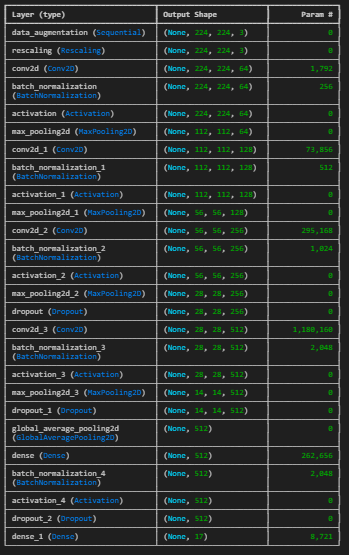
\includegraphics[width=0.65\textwidth]{images/cnn_model_summary.png}
    \caption{معماری و جزئیات لایه‌های شبکه‌ی عصبی \lr{CNN} پیاده‌سازی شده}
    \label{fig:model_summary}
\end{figure}

معماری این شبکه شامل چهار بلوک اصلی استخراج ویژگی و یک بخش طبقه‌بند نهایی است که کارکرد هرکدام به شرح زیر است:

\begin{itemize}
    \item \textbf{بلوک‌های کانولوشن (\lr{Conv2D}):} شبکه با ۶۴ فیلتر شروع شده و در لایه‌های عمیق‌تر تا ۵۱۲ فیلتر افزایش می‌یابد. لایه‌های اولیه الگوهای ساده (مثل لبه‌ها و رنگ‌ها) و لایه‌های عمیق‌تر، الگوهای پیچیده (مثل شکل گلبرگ‌ها) را تشخیص می‌دهند. 
    \item \textbf{نرمال‌سازی دسته‌ای (\lr{Batch Normalization}):} پس از هر لایه‌ی کانولوشن، این لایه توزیع داده‌ها را نرمال می‌کند. این کار نه تنها سرعت همگرایی را به‌شدت افزایش می‌دهد، بلکه نقش یک منظم‌ساز (\lr{Regularizer}) ملایم را نیز ایفا می‌کند.
    \item \textbf{جلوگیری از بیش‌برازش (\lr{Regularization \& Dropout}):} از آنجا که تعداد کل پارامترها حدود $1.8$ میلیون است، خطر حفظ کردن داده‌ها (\lr{Overfitting}) بسیار بالاست. به همین دلیل از جریمه‌ی \lr{L2} (با ضریب $10^{-4}$) در لایه‌های کانولوشن و لایه‌های \lr{Dropout} فزاینده (از $0.3$ تا $0.5$) در انتهای شبکه استفاده شد.
\end{itemize}

\begin{tipbox}[جایگزینی هوشمندانه‌ی \lr{Flatten} با \lr{Global Average Pooling}]
یکی از نقاط قوت این معماری، استفاده از لایه‌ی \lr{GlobalAveragePooling2D} پیش از لایه‌های متراکم (\lr{Dense}) است. اگر از \lr{Flatten} سنتی استفاده می‌کردیم، ابعاد خروجی بلوک آخر ($14 \times 14 \times 512$) به یک بردار $100,352$ تایی تبدیل می‌شد که به شدت تعداد پارامترها را بالا می‌برد. اما این لایه با میانگین‌گیری مکانی، آن را به یک بردار ۵۱۲ تایی فشرده می‌کند که علاوه بر کاهش چشمگیر محاسبات، از بیش‌برازش نیز جلوگیری می‌کند.
\end{tipbox}

\vspace{0.4cm}
\subsection{استراتژی آموزش و توابع فراخوان (\lr{Callbacks})}

مدل با بهینه‌ساز \lr{Adam} با نرخ یادگیری اولیه‌ی $0.001$ کامپایل گردید. برای کنترل هوشمند روند آموزش و رسیدن به بهترین وزن‌ها، توابع فراخوان زیر پیاده‌سازی شدند:

\begin{itemize}
    \item \textbf{\lr{ReduceLROnPlateau}:} در طول ۱۵۰ اپوک در نظر گرفته شده، هرگاه خطای اعتبارسنجی (\lr{val\_loss}) برای ۸ اپوک بهبود نیافت، نرخ یادگیری نصف شد. این اتفاق در اپوک‌های ۹، ۲۸، ۳۹، ۵۴، ۶۴ و ۷۲ رخ داد تا مدل بتواند دره‌های کمینه‌ی محلی را با قدم‌های کوچکتر طی کند.
    \item \textbf{\lr{EarlyStopping}:} آموزش شبکه پیش از رسیدن به اپوک ۱۵۰ و در اپوک ۷۶ متوقف شد؛ سپس بهترین وزن‌های مدل که متعلق به \textbf{اپوک ۵۶} (با حداقل \lr{val\_loss} برابر با $1.1234$) بود، بازگردانی شد تا از بیش‌برازش در اپوک‌های پایانی جلوگیری شود.
\end{itemize}

\begin{figure}[h!]
    \centering
    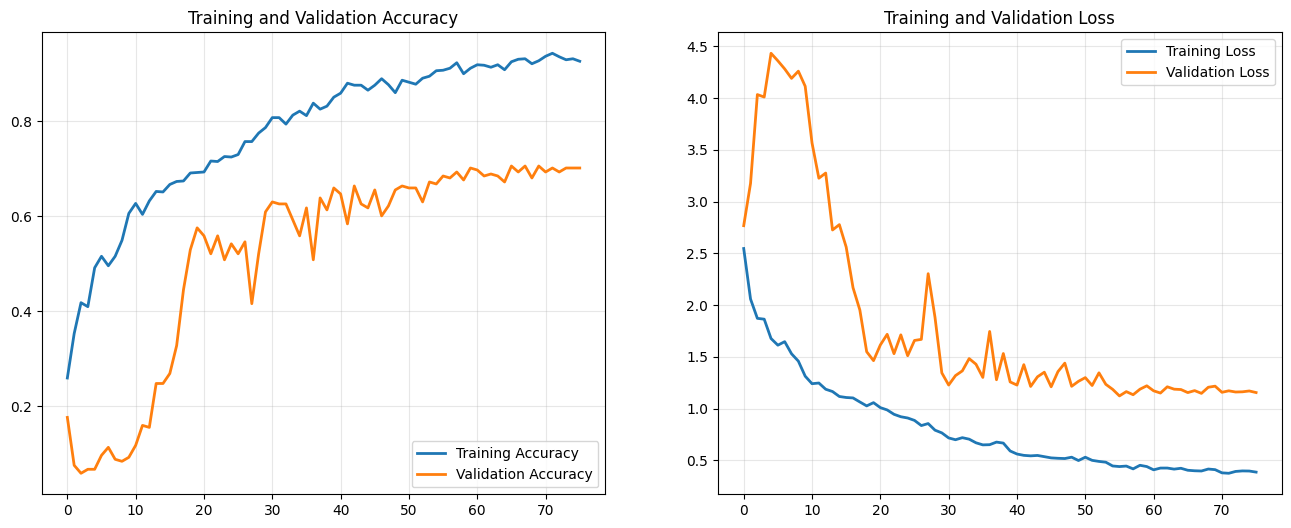
\includegraphics[width=0.95\textwidth]{images/cnn_history.png}
    \caption{روند تغییرات دقت (چپ) و تابع زیان (راست) مدل \lr{CNN} پایه در طول اپوک‌های آموزشی}
    \label{fig:cnn_history}
\end{figure}

\vspace{0.4cm}
\newpage
\subsection{ارزیابی نهایی روی داده‌های آزمون}

مدل بازگردانی شده (وزن‌های اپوک ۵۶) روی داده‌های آزمون (\lr{Test Set}) که کاملاً برای شبکه جدید بودند، ارزیابی شد و به \textbf{دقت $59.41\%$} و \textbf{خطای $1.5626$} دست یافت.

\begin{figure}[h!]
    \centering
    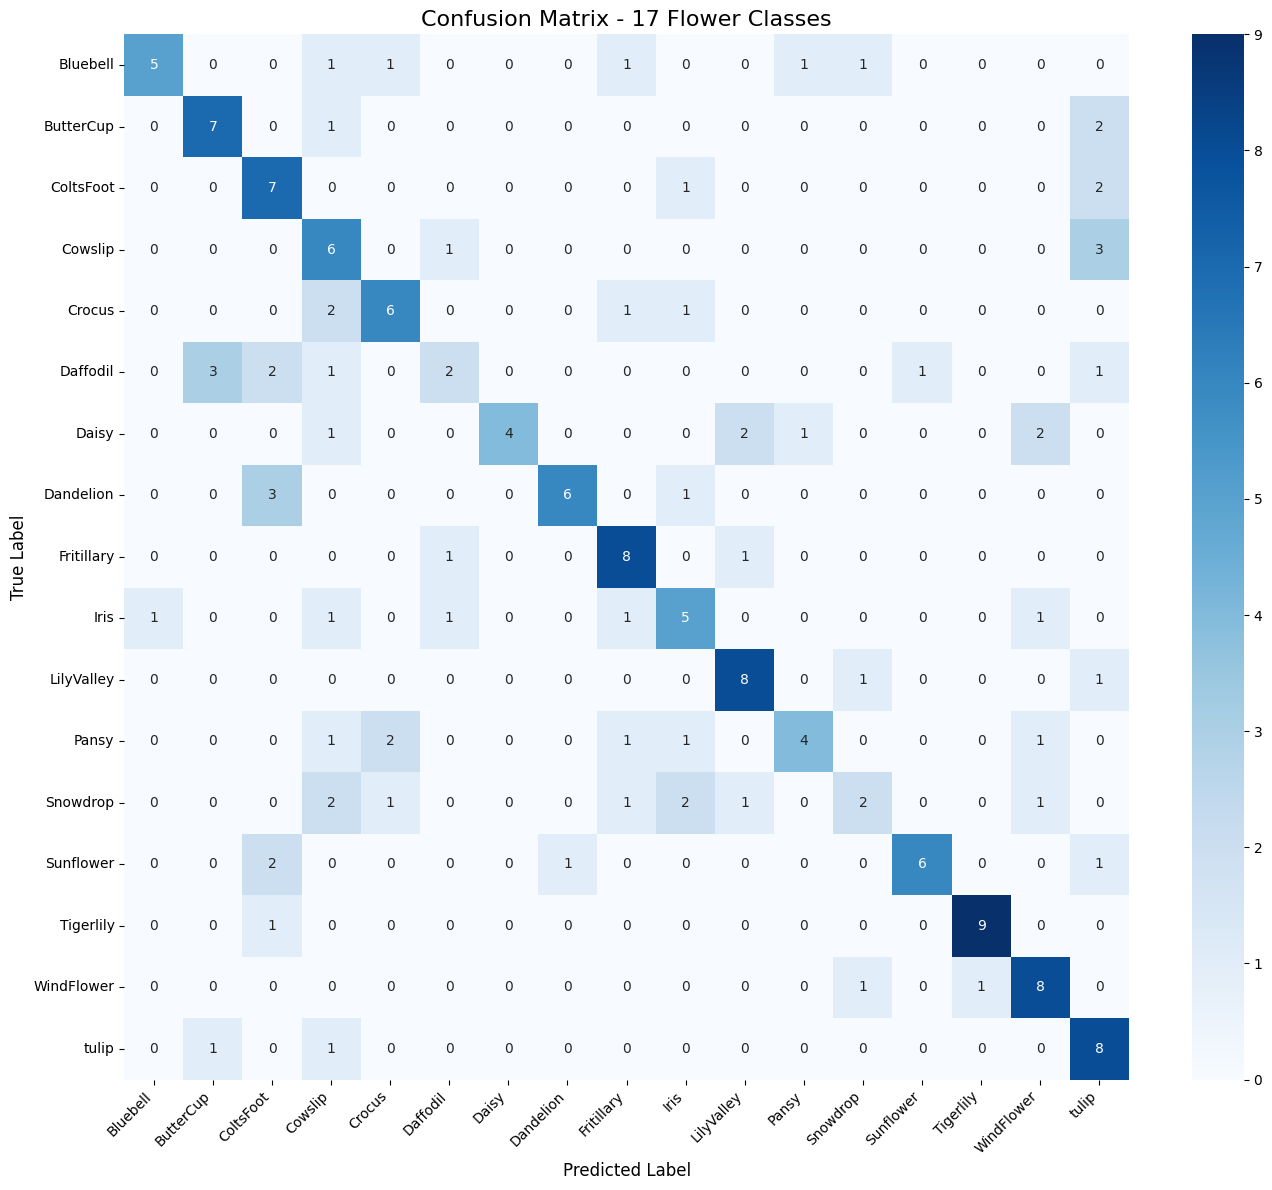
\includegraphics[width=0.85\textwidth]{images/cnn_conf_matrix.png}
    \caption{ماتریس درهم‌ریختگی عملکرد مدل روی ۱۷ کلاس تصویر}
    \label{fig:cnn_conf_matrix}
\end{figure}

\begin{notebox}[تحلیل گزارش دسته‌بندی (\lr{Classification Report})]
بررسی معیارهای ارزیابی در ماتریس درهم‌ریختگی نشان می‌دهد مدل روی کلاس‌هایی که ویژگی‌های بصری متمایزتری دارند، موفق‌تر عمل کرده است:
\begin{itemize}
    \item \textbf{بهترین عملکرد:} کلاس \lr{Tigerlily} (سوسن ببری) با \lr{F1-Score} برابر با $0.90$ دقیق‌ترین شناسایی را داشته است.
    \item \textbf{ضعیف‌ترین عملکرد:} کلاس‌های \lr{Daffodil} (نرگس) و \lr{Snowdrop} با \lr{F1-Score} بسیار پایین $0.27$ بیشترین خطای تشخیص را داشته و اغلب با سایر گل‌های هم‌خانواده اشتباه گرفته شده‌اند.
\end{itemize}
\end{notebox}

\vspace{0.4cm}
\newpage
\subsection{آزمون در شرایط واقعی (\lr{Inference})}

برای درک بهتر رفتار شبکه‌ی آموزش‌دیده، ۴ تصویر به صورت تصادفی از مجموعه‌ی تست به مدل داده شد تا پیش‌بینی نهایی و میزان اطمینان (\lr{Confidence}) خود را اعلام کند:

\vspace{0.3cm}
\begin{figure}[h!]
\centering
\begin{subfigure}{0.24\textwidth}
    \centering
    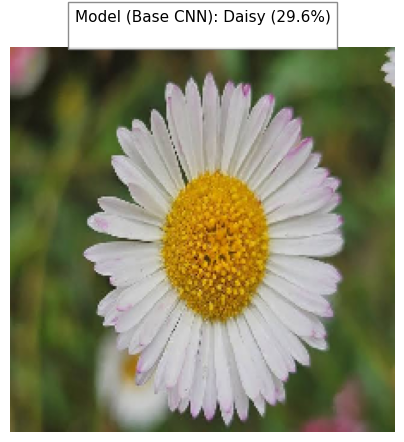
\includegraphics[width=\textwidth]{images/cnn_test1.png}
\end{subfigure}
\hfill
\begin{subfigure}{0.24\textwidth}
    \centering
    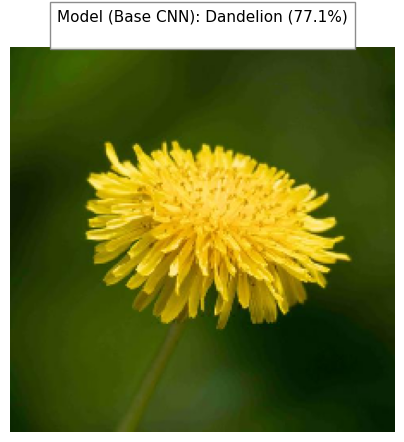
\includegraphics[width=\textwidth]{images/cnn_test2.png}
\end{subfigure}
\hfill
\begin{subfigure}{0.24\textwidth}
    \centering
    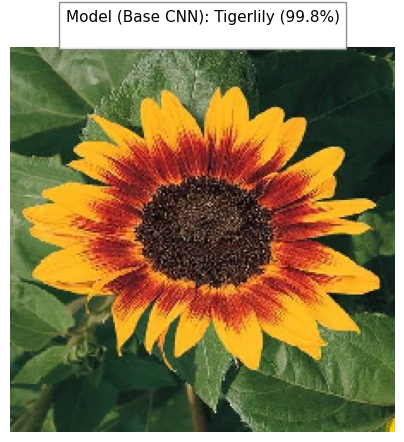
\includegraphics[width=\textwidth]{images/cnn_test3.png}
\end{subfigure}
\hfill
\begin{subfigure}{0.24\textwidth}
    \centering
    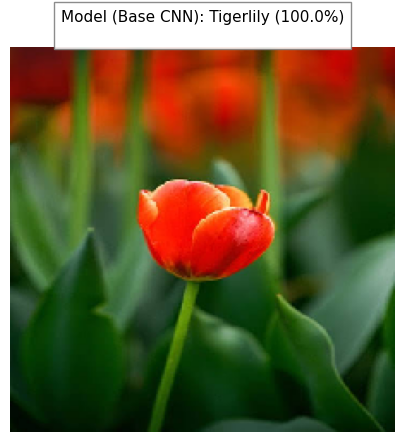
\includegraphics[width=\textwidth]{images/cnn_test4.png}
\end{subfigure}
\caption{نتایج پیش‌بینی مدل \lr{CNN} ساخته شده. (از چپ به راست: پیش‌بینی درست برای مینا و قاصدک / پیش‌بینی کاملاً غلط با اطمینان کاذب بالا برای آفتاب‌گردان و لاله)}
\label{fig:cnn_inference}
\end{figure}

\begin{warnbox}[تحلیل خطای طبقه‌بندی]
با وجود اینکه مدل کلاس‌های \lr{Daisy} و \lr{Dandelion} را به درستی تشخیص داد، اما در تصاویر آفتاب‌گردان (\lr{Sunflower}) و لاله (\lr{Tulip})، خروجی را با \textbf{اطمینان کاذب نزدیک به $100\%$} به عنوان \lr{Tigerlily} دسته‌بندی کرد! این پدیده نقطه‌ی ضعف کلاسیک مدل‌های آموزش‌دیده از پایه با داده‌ی کم است که ضرورت استفاده از مدل‌های ازپیش‌آموزش‌دیده (\lr{Pre-trained}) را بیش از پیش نمایان می‌سازد.
\end{warnbox}

\vspace{0.6cm}
\begin{notebox}[جمع‌بندی بخش اول و مسیر پیش‌رو]
همان‌طور که مشاهده شد، آموزش یک شبکه‌ی عصبی از پایه روی داده‌های محدود، با وجود به‌کارگیری تکنیک‌های مختلف، در نهایت به دقت $59.41\%$ ختم شد. همچنین در بررسی شرایط واقعی دیدیم که مدل در مواجهه با برخی کلاس‌ها دچار خطای همراه با «اطمینان کاذب» می‌گردد. 

برای غلبه بر این محدودیت‌ها، حل مشکل کمبود داده و ایجاد یک جهش چشمگیر در دقت دسته‌بندی، در \textbf{بخش بعدی} به سراغ تکنیک قدرتمند \textbf{یادگیری انتقالی (\lr{Transfer Learning})} خواهیم رفت تا این مسئله را به شکلی کاملاً بهینه‌تر و با بهره‌گیری از شبکه‌های ازپیش‌آموزش‌دیده حل کنیم.
\end{notebox}